\documentclass{article}
\usepackage{graphicx}
\title{Surfaces}
\author{Evan Sadler}

\begin{document}
\maketitle

\section{Introduction}
The purpose of this document is to provide introduction to my project. The document will consist of motivation, interesting examples, and the short-comings of the classes. The focus is primarily on the Surface_Revolution() class. 


\section{Motivation}
Differential geometry is a very visual field of mathematics. It examines inherent properties of surfaces by using a lot of linear algebra and calculus. Studying differential geometry requires interpeting complicated notation and a vivid imagination. This paired with a lack of visual aids makes Math 442 an unecessesarily difficult course. The goal of my project is to provide students with a resource for checking work and visual aids more than just plot3d(). 

\section{Examples}

\subsection{Torus}
The following example was homework problems from math 442 that can be solved using my program: \\

The torus was commonly used as an example in math 442. It is essentially the surfaces of a doughnut. In homework 6 problem 3, we were asked to find the different types of points on a torus. Interpreting the mathematics is very demanding, however the intuition is quite simple. Unfortunately, no visual aid existed to help grasp the intuition. My Surface\_Revolution() class contains the PlotPoints() function, which provides the required help.

Code: 
\begin{enumerate}
\item s = Surface\_Revolution(3+cos(v), sin(v))
\item s.PlotPoints(100)
\end{enumerate} 

\textit{Look at Figure 1 before reading the next paragraph!} \\ \\
The torus has three out of four types of points, which are color cordinated. In order to explain the significance of each type, I will need you to use your imagination! Imagine that the torus is oriented like a wheel on a car. Now imagine your are really small and standing on top of the wheel (on the blue part of the torus). Take your left foot and step it in any direction. Your left foot will land below your right foot. This is because the surface curves in one direction away from the point. In this case, it the surface is curving towards the ground. This is called an elliptic point after an ellipse because ellipses only have elliptical points. If you are standing on the green section, parts of the surface curve away from you and others curve towards you. If you were a hamster running inside the torus, you could run "up" and make a loop or on the other hand, fall off the side. These points are called hyperbolic because hyperbolas are characterized by these types of points. Finally, image you set the torus down like an intertube floating on water. If you were very small and walked along the red line, your altitute would stay completely flat. However, any deviation from the red line would surely lead to your doom as you would fall off the tube. This  points are called parabolic. This is difficult for me to explain, and I apologize if it makes little sense. It is the best I can do!



\begin{figure}[ht!]
\centering
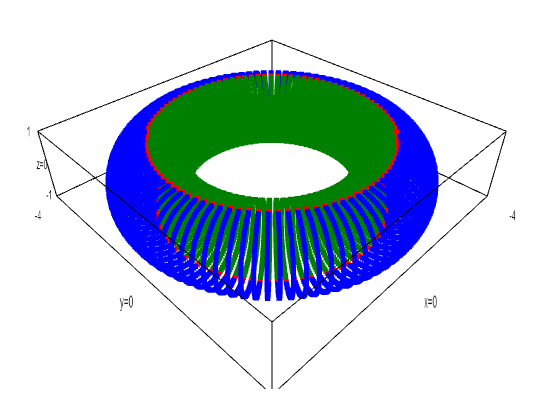
\includegraphics[width=90mm]{torus.png}
\caption{torus by point type}
\label{}
\end{figure}

\subsection{One-Sheeted Hyperboloid}

A One-Sheeted hyperoboloid contains only hyperbolic points. Using $a=0.5$ and $c=10$ provides an illustrative graph.


\begin{enumerate}
\item s = Surface\_Revolution(0.5*cosh(v),10*v)
\item s.PlotPoints(100)
\end{enumerate}

\subsection{Cone}

A cone contains only parabolic points. Using $a=0.5$ and $c=1$ provides a cone where this is very apperent. 

\begin{enumerate}
\item s = Surface\_Revolution(0.5*v),v)
\item s.PlotPoints(100)
\end{enumerate}

\subsection{Other}
Both classes contain functions that can be used to check various properties of a surface. I did not include examples in this document as explanations are without easy intuition. But, I encourage you to play around with the other functions using the provided examples in the sage worksheet.

\section{Improvements}
As a novice programmer, I left plently of room for improvement. First of all, Sage is limited in terms of symbolic calculation. This leaves some of the symbolic answers in a more convfusing state than necessary. Also, this class only works for "smooth surfaces" and no part of my class checks to see the inputted surface is in fact, smooth. Thus, it is prone to error. Finally, there is no PlotPoints() function for the Surface_Two_Variables() class. The computation was incredible slow and demanding of Sage. There exist ways to speed up calculations and graph the points, however it was far beyond the scope of my programming abilities and required too much time to learn on my own.

\section{Conclusion}
Thank you for taking the time to review my project and read through the document.

\end{document}